\documentclass{../industrial-development}
\graphicspath{{6-interaction-inside-and-outside-team/}}

\title{Команда разработчиков: взаимодействие внутри и вне команды}
\author{Смирнов Дмитрий Владиславович, ПИЭ-21 МО}
\date{}

\begin{document}

\begin{frame}
  \titlepage
\end{frame}


\section{Взаимодействие внутри команды}

\subsection{Вертикальная форма взаимодействия сотрудников}

\begin{frame} \frametitle{Вертикальная форма взаимодействия сотрудников}
  \begin{block}{Определение}
\alert{Вертикальная (линейная) форма взаимодействия} "--- это~форма взаимодействий иерархического типа, у которой во главе каждого звена или подразделения стоит единоличный руководитель, наделенный всем объемом полномочий и власти
  \end{block}
\end{frame}

\lecturenotes
Вертикальная (линейная) форма взаимодействия –  это простейшая форма взаимодействий иерархического типа, характеризующаяся тем, что во главе каждого звена или подразделения стоит единоличный руководитель, наделенный всем объемом полномочий и власти. 

 Вертикальная форма взаимодействий имеет структуру подчиненности от верхнего уровня к нижнему. Существует четко определенная цепочка командования с вертикальной организацией, и человек в верхней части организационной структуры имеет наибольшую власть. Сотрудники отчитываются перед лицом непосредственно над ними в организационной структуре. Каждый человек несет ответственность за определенную область или набор обязанностей.

\begin{frame} \frametitle{Схема вертикальной формы взаимодействия}
	\begin{block}{}
		\centerline{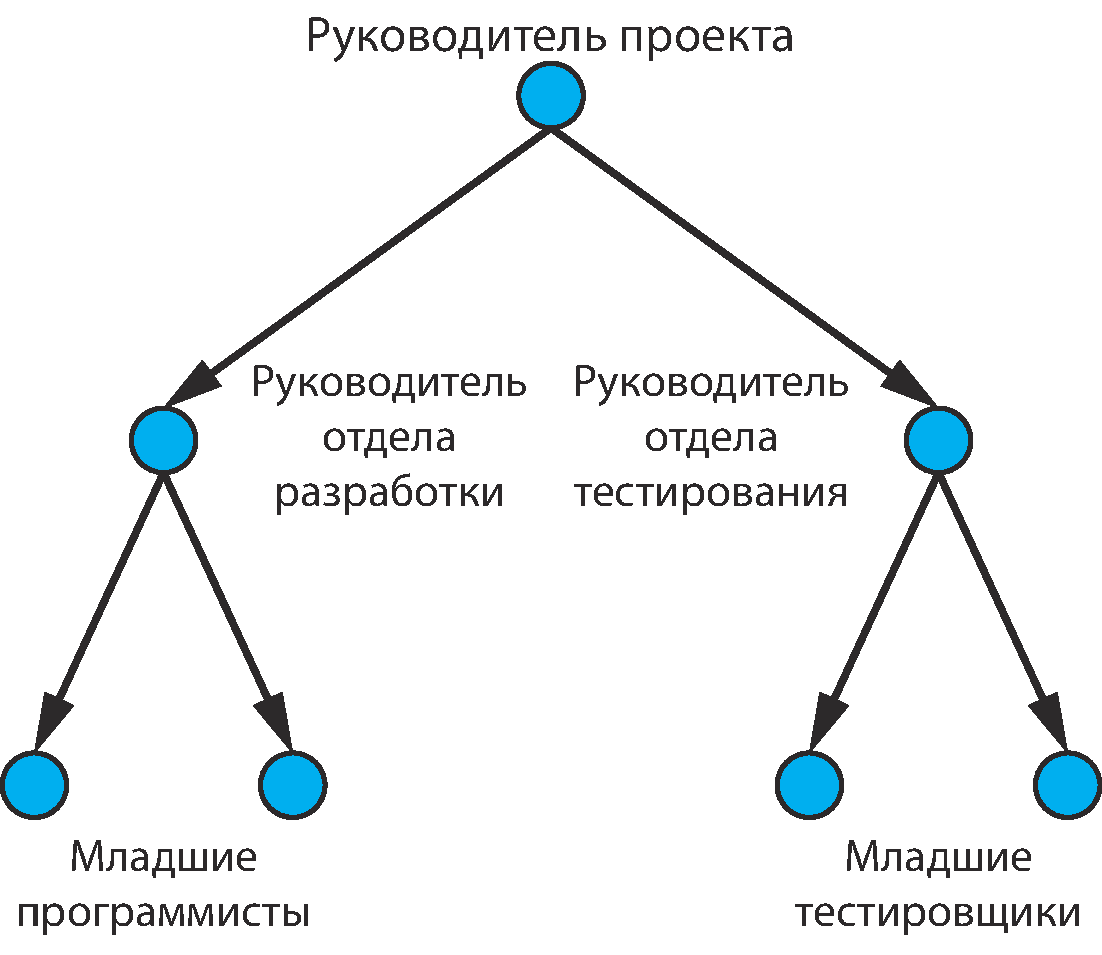
\includegraphics[height=0.7\textheight]{vertical.pdf}}
	\end{block}
\end{frame}

\lecturenotes
Пример вертикальной формы взаимодейтсвия в ИТ компании:
1ый уровень - руководитель компании
2ой уровень - исполнительный директор (отвечает за ведение проектов) и коммерческий директор (отвечает за продажи)
3й уровень - менеджеры проектов и менеджеры продаж.

Также можно рассмотреть другой вариант данной формы взаимодействия в ИТ команде:
1ый уровень -  технический директор
2ой уровень -  руководитель отдела разработки и руководитель отдела тестирования
3ий уровень - программисты и тестировщики


\begin{frame} \frametitle{Преимущества вертикальной формы взаимодействия}

  
  \begin{itemize}
  \item Удобное распределение задач
  \item Простота управления
  \item Возможность роста по карьерной лестнице
  \item Четко выраженная ответственность
  \item Высокий уровень специализации профессиональной деятельности

  \end{itemize}
\end{frame}


\begin{frame} \frametitle{Недостатки вертикальной формы взаимодействия}
  
  \begin{itemize}
  \item Медленное общение между отделами и сотрудниками
  \item Концентрация полномочий на верхнем уровне управления
  \item Большая физическая и моральная нагрузка на руководителей
  \item Отсутствие инициативы среди сотрудников низших звеньев
  \end{itemize}
\end{frame}

\subsection{Горизонтальная форма взаимодействия сотрудников}

\begin{frame} \frametitle{Горизонтальная форма взаимодействия сотрудников}
  \begin{block}{Определение}
\alert{Горизонтальная форма взаимодействия} "--- это форма взаимодействий между сотрудниками, занимающими равное положение в организации, как внутри отдела, так и между отделами
  \end{block}
\end{frame}

\lecturenotes
Горизонтальные связи — это связи между двумя или более равными по положению в иерархии или статусу членами команды. Каждый сотрудник имеет аналогичный вклад в то, как работает организация. Они могут выполнять множество различных функций и могут отчитываться перед несколькими руководителями, а не одним начальником. Например, руководители проектов или руководители групп отчитываются перед командой руководителей, причем члены каждой команды по существу равны с точки зрения власти.

\begin{frame} \frametitle{Схема горизонтальной формы взаимодействия}
  \begin{block}{}
\centerline{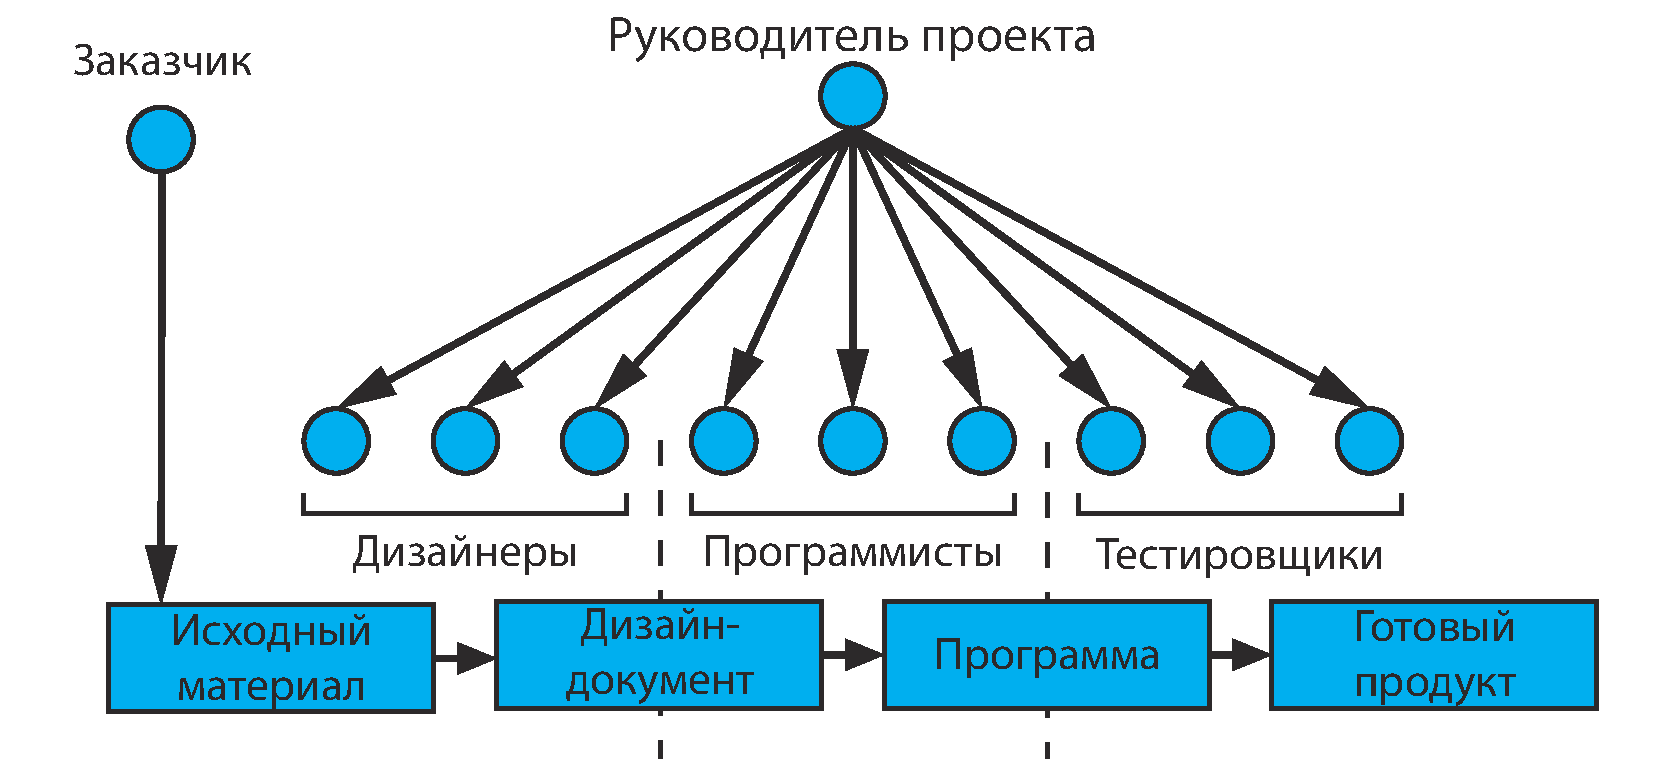
\includegraphics[width=1\textwidth]{horizontal.pdf}}
  \end{block}
\end{frame}

\begin{frame} \frametitle{Преимущества горизонтальной формы взаимодействия}
  
  \begin{itemize}
  \item Высокий моральный дух сотрудников, поскольку они имеют больше полномочий на принятие решений
  \item Более активное сотрудничество с клиентами благодаря большей вовлечённости сотрудников в проект
  \item Открытый контакт сотрудников друг с другом
  \item Возможность принятия совместных решений
  \end{itemize}
\end{frame}

\begin{frame} \frametitle{Недостатки горизонтальной формы взаимодействия}
	
	\begin{itemize}
		\item Отличия в терминологии и точке зрения
		\item Тенденция считать свой участок работы самым важ­ным, что часто препятствует эффективному взаимодей­ствию сотрудников
		\item Риск принятия решений, не удовлетворяющих интересам организации в целом
	\end{itemize}
\end{frame}

\lecturenotes
- Различия в термнологии и точке зрения, присущие каждому отде­лу и часто непонятные представителям других отделов, вы­ступающих в роли получателей информаци
- довольно распространен­ная тенденция считать свой участок работы самым важ­ным, что часто препятствует эффективному взаимодей­ствию сотрудников
- опасность того, что отделы А и Б могут на низком уровне принять решение, которое не отвечает интересам организации в целом

\subsection{Матричная форма взаимодействия сотрудников}

\begin{frame} \frametitle{Матричная форма взаимодействия сотрудников}
  \begin{block}{Определение}
	\alert{Матричная форма взаимодействия} "--- решетчатая структура, базирующаяся на принципе  двойного подчинения: функционального и проектного
  \end{block}
\end{frame}

\lecturenotes
Матричная структура представляет собой комбинацию двух видов разделения: по функциям и по продукту. Она построенна на основе принципа двойного подчинения исполнителей: с одной стороны, непосредственному руководителю функционального подразделения, которое предоставляет персонал руководителю проекта, с другой стороны  - руководителю временной группы, который наделен необходимыми полномочиями для осуществления процеса управления и несет ответственность за сроки и ресурсы.

\begin{frame} \frametitle{Функциональная и проектная организация управления}
	\begin{block}{Определение}
		\alert{Функциональная организация управления} "--- вертикальная форма взаимодействия сотрудников, в которой распределение работ происходит по функциональным областям
	\end{block}
	\begin{block}{Определение}
		\alert{Проектная (дивизиональная) организация управления} "--- вертикальная форма взаимодействия сотрудников, в которой распределение работ происходит по выпускаемой продукции или по регионам
	\end{block}
\end{frame}

\begin{frame} \frametitle{Схема матричной формы взаимодействия}

\begin{block}{}
	\centerline{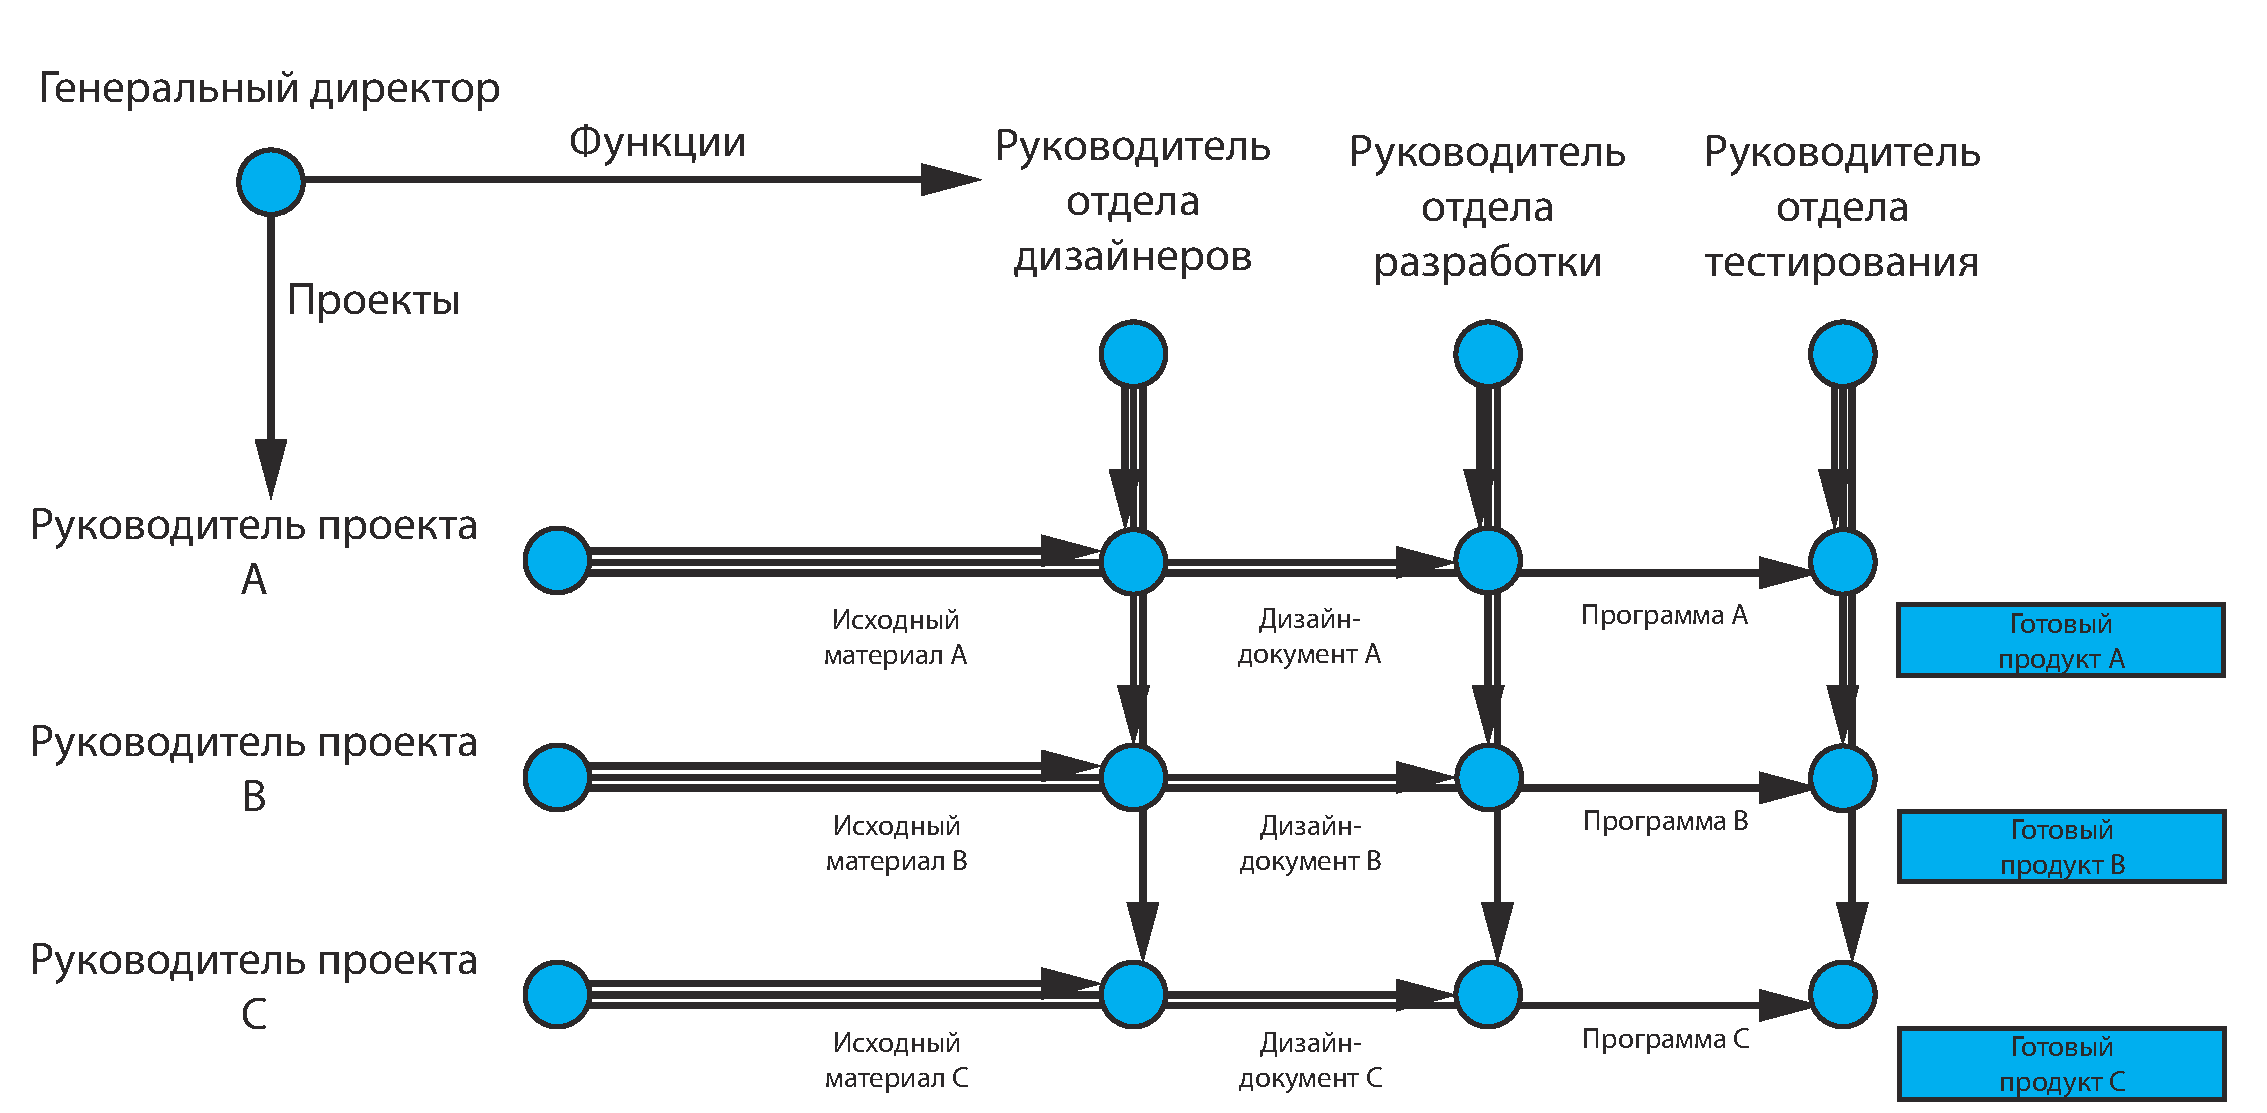
\includegraphics[width=1\textwidth]{matrix.pdf}}
\end{block}

\end{frame}

\lecturenotes
Матричные структуры охватывают не всю организацию, а лишь ее часть. Причем успех в значительной мере зависит от того, в какой степени руководители проектов обладают профессиональными качествами менеджеров и способны выступить в проектной группе в роли лидеров.
Руководители проектов в матричной структуре отвечают в целом за интеграцию всех видов деятельности и ресурсов, относящихся к данному проекту. Для того, чтобы они смогли добиться этого, все материальные и финансовые ресурсы по данному проекту передаются в их полное распоряжение. Руководители проектов сохраняют за собой право определять приоритетность и сроки решения той или иной задачи, в то время как руководители структурных подразделений могут лишь выбирать конкретного исполнителя и методику решения.
Матричные формы взаимодействий очень активно используются в IT  командах

\begin{frame} \frametitle{Преимущества матричной формы взаимодействия}
  
  \begin{itemize}
  \item Сокращение нагрузки на руководителей высшего уровня управления 
  \item Получение высококачественных результатов по большому количеству проектов
  \item Активизация деятельности руководителей и работников управленческого аппарата
  \item Усиление личной ответственности конкретного руководителя за его проект
  \end{itemize}
\end{frame}

\begin{frame} \frametitle{Преимущества матричной формы взаимодействия}
  
  \begin{itemize}
 \item Гибкость выполнения работ по всем проектам
 \item Эффективное использование ресурсов
 \item Адаптивность к нагрузкам по проектам
 \item Четкое разграничение по проектам
 \item Активное взаимодействие со всеми заказчиками
  \end{itemize}
\end{frame}

\lecturenotes
Преимущества матричной формы
- Сокращение нагрузки на руководителей высшего уровня управления путем передачи полномочий принятия решений на средний уровень при сохранении единства координации и контроля за ключевыми решениями на высшем уровне
- Получение высококачественных результатов по большому количеству проектов
- Активизация деятельности руководителей и работников управленческого аппарата в результате формирования проектных команд, активно взаимодействующих с функциональными подразделениями
- Усиление личной ответственности конкретного руководителя как за проект в целом, так и за его элементы (в частности за трудовые ресурсы)
- Достижение большей гибкости выполнения работ по всем проектам
- Эффективное использование ресурсов
- Гибкость и адаптивность к нагрузкам по проектам
- Четкое разграничение по проектам
- Проект находится в центре внимания - клиент доволен

\begin{frame} \frametitle{Недостатки матричной формы взаимодействия}
  
  \begin{itemize}
  \item Сложность матричной структуры для практической реализации
  \item Возникновение конфликтов между руководителями проектной и функциональной структурами из-за системы двойного подчинения
  \item Двусмысленность роли исполнителя и его руководителей
  \item Неопределённость властных полномочий среди руководителей
  \item Частичное дублирование функций
\end{itemize}
\end{frame}

\lecturenotes
Недостатки матричной формы
- Сложность матричной структуры для практической реализации, для ее внедрения необходима длительная подготовка работников и соответствующая организационная культура
- В связи с системой двойного подчинения подрывается принцип единоначалия, что часто приводит к конфликтам между менеджерами функиональных подразделений и управляющими проектов, между проектной и функциональной структурами. Появляется возможность острых противоречий между сторонами матрицы.
- В рамках этой структуры порождается двусмысленность роли исполнителя и его руководителей, что создает напряжение в отношениях между членами трудового коллектива компании
- Характерна борьба за власть, так как в ее рамках четко не определены властные полномочия
- Наблюдается частичное дублирование функций

\begin{frame} \frametitle{Недостатки матричной формы взаимодействия}
\begin{itemize}
  \item Несвоевременное принятие управленческих решений
  \item Отсутствие традиционной системы взаимосвязей между подразделениями
  \item Неоднозначное определение приоритетов по проектам
  \end{itemize}
\end{frame}

\lecturenotes
Недостатки матричной формы
- Несвоевременно принимаются управленческие решения - характерно групповое принятие решений
- Нарушается традиционная система взаимосвязей между подразделениями
- Каждая из проектных групп будет тянуть одеяло на себя – возникнут проблемы  с определением приоритетов

\section{Взаимодействие команды с внешней средой}

\subsection{Определение внешней среды}
\begin{frame} \frametitle{Внешняя среда}
	\begin{block}{Определение}
		\alert{Внешняя среда} "--- это совокупность различных субъектов, условий, структур и факторов, действующих в окружении предприятия и влияющих на различные сферы его деятельности.
	\end{block}
\end{frame}

\lecturenotes Внешняя среда "--- это совокупность активных хозяйствующих субъектов, экономических, общественных и природных условий, национальных и межгосударственных институциональных структур и других внешних условий и факторов, действующих в окружении предприятия и влияющих на различные сферы его деятельности

\begin{frame} \frametitle{Внешние участники}
	\begin{itemize}
		\item Инициатор проекта
		\item Спонсор (куратор) проекта
		\item Заказчик
		\item Инвесторы
		\item Потребители конечной продукции проекта
		\item Поставщики
		\item Конкуренты
		\item Органы власти
		\item Лицензоры
		\item Консалтинговые и юридические организации 
		\item Генеральный подрядчик
		\item Субконтракторы
		\item Проектировщики
		\item Собственники земли
	\end{itemize}
\end{frame}

\lecturenotes
- Инициатор проекта - в качестве инициатора может выступать практически любой из будущих участников проекта. Он выдвигает главную идею, готовит предварительное обоснование и предложения по осуществлению проекта. Но деловая инициатива по осуществлению проекта, в конечном счете, принадлежит заказчику или владельцу проекта.

- Спонсор (куратор) проекта – лицо внутри или вне организации, обеспечивающее финансовые ресурсы проекта. Это лицо, которое осуществляет не только финансовую поддержку, но также любую административную или организационную поддержку проекта. Как правило, спонсором является менеджер высшего звена организации, исполняющей проект. Спонсор: определяет приоритеты проекта, обеспечивает проект ресурсами, обеспечивает взаимодействие с функциональными подразделениями, рассматривает и утверждает запросы на изменения. Во внутренних проектах может нести конечную ответственность за результаты проекта.

- Заказчик - будущий владелец проекта и потребитель его результатов. Он определяет основные требования к проекту и обеспечивает его финансирование за счет своих либо привлеченных от спонсоров или инвесторов средств. Он же заключает контракты с основными исполнителями проекта и управляет процессами взаимодействия между всеми участниками проекта. Иногда под термином владелец проекта подразумевается не организация-заказчик в целом, а отдельное лицо в этой организации или группа лиц, обличенные достаточной властью и кровно заинтересованные в успешном выполнении проекта. В этом случае функцией владельца проекта будет «политическая поддержка» ваших действий как менеджера проекта при контактах с организацией-заказчиком, а также сглаживание потенциальных конфликтов с другими группами, лоббирующими свои интересы или интересы Ваших конкурентов.

- Инвесторы - банки, инвестиционные фонды, другие организации или физические лица, которые вкладывают средства в проект с целью получения на вложенные инвестиции максимально возможной прибыли. Инвесторы заключают соответствующие контракты с заказчиком, а затем контролируют их выполнение и осуществляют необходимые расчеты с другими участниками проекта по мере его реализации.

- Потребители конечной продукции проекта - это может быть как сам заказчик, так и различные организации и физические лица, являющиеся покупателями конечной продукции проекта. Они определяют требования к производимой продукции и оказываемым услугам. От их поведения зависит возмещение затрат и прибыль от проекта.

- Поставщики - организации, осуществляющие поставки для проекта материалов, оборудования, транспортных средств и т.д. на контрактной основе.

- Конкуренты основных участников проекта.

- Органы власти - представители местных, региональных и центральных органов власти, контролирующие выполнение определенных государственных и общественных требований к проекту.

- Лицензоры - организации, выдающие лицензии на право выполнения определенных видов работ и услуг, ведение торгов, на право владения земельным участком и т.д.

- Консалтинговые, инжиниринговые, юридические организации , вовлеченные в процесс осуществления проекта.

- Общественные группы и организации, население, чьи значимые интересы затрагивает реализация проекта.

- Генеральный подрядчик- участник проекта, который заключает основной контракт с заказчиком (инвестором) и договора с внешними исполнителями.

- Субконтракторы.- участники проекта, входящие в договорные отношения с контратором более высокого уровня и отвечающие за определенные виды работ или услуг.

- Проектировщики.

- Собственники земли.

\subsection{Взаимодействие с заказчиками}
\begin{frame} \frametitle{Этапы выстраивания отношений с~заказчиками}
	\begin{block}{Определение}
		\alert{Заказчик} "--- это человек или группа людей, которые определяют и согласовывают целевые показатель уровня услуги
	\end{block}
\end{frame}
	
\lecturenotes
Заказчик для Поставщика ИТ-услуг — это человек или группа людей, которые работают в интересах иного, по отношению к поставщику ИТ услуг, бизнеса; определяют и согласовывают целевые показатели уровня услуги. Термин «Заказчики» также иногда используется для обозначения пользователей, например, в контексте «клиентоориентированной организации».


\begin{frame} \frametitle{Этапы выстраивания отношений с заказчиками}

\begin{itemize}
 \item Знакомство с клиентом
 \item Установление взаимоотношений
 \item Составление договора и ТЗ
 \item Информирование заказчика о технологии ведения проекта
 \item Сбор команды на проект 
 \item Старт проекта 
 \item Мониторинг хода работы по проекту
 \item Сдача работ
 \item Постпроектные взаимоотношения
  \end{itemize}
\end{frame}

\lecturenotes
1. Знакомство с клиентом
  - сбор информации о компании
  -  выяснение потребностей клиента
  - предоставление оценочной стоимости за данную работу
 -  выяснение, готов ли клиент столько платить (естественно сразу никто не назовет конкретных сумм, но если проект приблизительно оценивается в 3-5 миллионов, а потенциальный заказчик считает, что миллион –  это очень много, то, наверное, у вас с ним ничего не получится)
  - формирование вывода: подходит ли такой клиент Вам или нет
2. Установление взаимоотношений
3. Составление договора и ТЗ.
4. Информирование заказчика о технологии ведения проекта
 - какие технологии будут использоваться
 - кто за что отвечает
 - кто что делает
 - для чего делаются те или иные действия
 Это необходимо для решения проблемных вопросов о задержках сроков или изменения бюджета.
5. Далее следует собрать команду на проект: назначить менеджера проекта и определиться с командой разработчиков.
6. Старт проекта.
7. Мониторинг хода работы по проекту. 
На данном этапе у клиента могут появиться желания по доработке/изменению программы или какого-либо функционала. Чтобы избежать конфликта с клиентом, менеджеру проекта приходится объяснять, что эти правки могут отразиться на сроках сдачи продукта, а также может измениться его стоимость, поскольку данные правки займут n-ое количество часов и их надо будет оплатить. В конце концов, клиент с нами соглашается и либо отказывается от своего пожелания, либо оплачивает дополнительные часы. 
8. Сдача работ.
На данном этапе следует добиться сдачи работ в полном соответствии с правилами, установленными в соответствующих документах, которые подписанным клиентом.
9. Постпроектные отношения. 
На данном этапе стоит добиться заключения договора на техническое обслуживания продукта.

\begin{frame} \frametitle{Проблемы взаимодействий с заказчиками}
	Со стороны заказчика:
	\begin{itemize}
		\item Недостаток интереса к проекту
		\item Нехватка лидерских навыков, политического опыта, времени или энергии, чтобы довести проект до логического завершения
		\item Уклонение от расстановки приоритетов
		\item Неопределённые критерии успеха / завершения проекта
	\end{itemize}
\end{frame}

\begin{frame} \frametitle{Проблемы взаимодействий с заказчиками}
	С обеих сторон:
	\begin{itemize}
		\item Плохие коммуникации и медлительность
		\item Благодушие ("No-Bad-News" Environment)
		\item Потеря интересов участников проекта в его завершении
		\item Слабое управление требованиями
		\item Нереалистично рассчитанный бюджет
	\end{itemize}
\end{frame}

\begin{frame} \frametitle{Проблемы взаимодействий с заказчиками}
	Со стороны команды:
	\begin{itemize}
		\item замалчивание трудностей, с которыми столкнулась команда
		\item недостаток или отсутствие управления рисками
		\item недостаточно ясные процессы контроля и управления изменениями
	\end{itemize}
\end{frame}

\subsection{Взаимодействие с подрядчиками}
\begin{frame} \frametitle{Взаимодействие с подрядчиками}
	\begin{block}{Определение}
		\alert{Подрядчик} "--- лицо, выполняющее работы по договору подряда или государственному контракту, заключаемым с компанией-заказчиком
	\end{block}

	\begin{block}{Виды подрядчиков}
		\begin{itemize}
			\item Поставщики аппаратно-программных средств
			\item Провайдеры
			\item Проектировщики
		\end{itemize}
	\end{block}
\end{frame}

\lecturenotes
Под подрядчиком в ИT понимается физические и юридические лица, которые выполняют работы по договору подряда или государственному контракту, заключаемым с заказчиками в соответствии с ГК РФ. Подрядчики обязаны иметь лицензию на осуществление ими тех видов деятельности, которые подлежат лицензированию в соответствии с федеральным законом.

Цель процесса управления подрядчиками является управление подрядчиками и услугами, которые они поддерживают, а также постоянное обеспечение требуемого качества предоставления ИТ-услуг бизнесу, включая получения эффективной отдачи от вложенных в подрядчика денег.

Виды подрядчиков:
- Поставщики аппаратно-программных средств (Вендоры, разработчики; Разработка, внедрение, тестирование, сопровождение ПО и аппаратного комплекса)
- Провайдеры (Интернет-провайдеры, телекоммуникационные компании; Предоставление телекоммуникационных услуг (телефония, интернет, сетевое окружение))
- Проектировщики (Системные интеграторы, IT-консалтинг компании; Проектирование и аудит сетевых коммуникаций, архитектуры, базы данных, системы пользовательских приложений, системы безопасности, системы управления (инжиниринг))

\begin{frame} \frametitle{Проблемы взаимодействий с подрядчиками}
	Со стороны подрядчика:
	\begin{itemize}
		\item Срыв сроков 
		\item Некачественная работа
		\item Невнимание к ТЗ
		\item Отсутствие требуемого опыта
		\item Применение старых технологий
		\item Снижение мотивации
		\item Неспособность быстро решить возникшую проблему
  	\end{itemize}
\end{frame}

\lecturenotes
Если в штате компании не хватает программистов, и имеется большое количество задач по проектам, то можно нанять подрядчика. В качестве его могут выступать как и фрилансеры, так и другие компании. Конечно же, в этом все равно есть определенные риски, и поэтому следует выбирать подрядчика очень внимательно. 

\begin{frame} \frametitle{Проблемы взаимодействий с подрядчиками}
	Со стороны команды:
	\begin{itemize}
		\item Неопредленность цели деятельности
		\item Постоянная смена задач и требований
		\item Нежелание оплачивать услуги подрядчика
		\item Отсутствие необходимых компетенций и навыков  в базовых вещах, таких как – обыкновенная логика, бизнес-знаниях и т.п.
	\end{itemize}
\end{frame}

\lecturenotes
- Неопредленность – когда руководство заказчика, в общем то и понимает – что-то делать надо, а вот, что – обозначить не может. Если цель неопределенна, то достичь ее невозможно. Причин тому множество: мало знаний у самого заказчика, неверное делегирование нерадивым сотрудникам, отсутсвие внятных бизнесс-процессов в компании – например, задачи it-отдела размазаны по ряду других и много другое.
- Постоянная смена задач и требований, даже если есть план работ, зачастую заказчики по 5 раз за неделю меняют приоритеты – сначала давайте делать это, потом вот это и т.д. Если появилась необходимость оперативного внедрения, изменения, разработки, то необходимо оговорить с подрядчиком данный вопрос отдельно. Так чтобы основной процесс шел, а форс-мажорный реализовывался дополнительными силами.
- Финансы – Заказчик либо вовсе не желает платить, либо делает это так нерегулярно, с такими задержками и проволочками, что становится понятно – компания-подрядчик попусту тратит свои ресурсы не зарабатывая.
- Отсутствие необходимых компетенций и навыков в базовых вещах, таких как – обыкновенная логика, бизнес-знаниях и т.п. 

\subsection{Бета-тестирование}
\begin{frame} \frametitle{Бета-тестирование}
	\begin{block}{Определение}
		\alert{Бета-тестирование} "--- это интенсивное использование почти готовой версии продукта с целью выявления максимального числа ошибок в его работе
	\end{block}
\end{frame}

\lecturenotes
Бета-тестирование - это интенсивное использование почти готовой версии продукта (как правило, программного или аппаратного обеспечения) с целью выявления максимального числа ошибок в его работе для их последующего устранения перед окончательным выходом продукта на рынок, к массовому потребителю.

\begin{frame} \frametitle{Бета-тестирование}
	\begin{itemize}
		\item Закрытое бета-тестирование
		\item Открытое бета-тестирование
	\end{itemize}
\end{frame}

\lecturenotes
- Закрытое бета-тестирование - программа тестируется в небольшой группе пользователей по приглашениям.
- Открытое бета-тестирование - любой пользователь сможет присоединиться к открытому бета-тестированию и отправить личный отзыв. Этот вариант позволяет протестировать приложение в большей группе и получить большой объем обратной связи.

\begin{frame} \frametitle{Преимущества бета-тестирования}
	\begin{itemize}
		\item Снижает риск выхода продукта из строя посредством валидации клиента
		\item Повышает качество продукции благодаря обратной связи с клиентами
		\item Создает доброжелательность с клиентами и повышает удовлетворенность клиентов
		\item Позволяет компании тестировать инфраструктуру после запуска продукта
	\end{itemize}
\end{frame}

\begin{frame} \frametitle{Недостатки бета-тестирования}
	\begin{itemize}
		\item Отсутствие контроля тестирования со стороны компании
		\item Поиск правильных бета-тестеров и поддержание их участия
	\end{itemize}
\end{frame}

\lecturenotes
Управление тестированием – проблема. По сравнению с другими типами тестирования, которые обычно выполняются внутри компании в контролируемой среде, бета-тестирование выполняется в реальном мире, где у компании редко есть контроль.

\subsection{Эксперт в предметной области}
\begin{frame} \frametitle{Эксперт в предметной области}
	\begin{block}{Определение}
		\alert{Эксперт в предметной области} "--- это человек со специальными знаниями в конкретной области деятельности
	\end{block}
\end{frame}
\lecturenotes
Эксперт в предметной области - это человек со специальными знаниями в конкретной области деятельности. Как правило, это сотрудник с глубоким пониманием определенных бизнес-функций или операций, зачастую с многолетним опытом непосредственного в них участия. Также этот термин применяется к сотрудникам, имеющим глубокие познания в области IТ, производстве, управлении поставками или других областях деятельности.
Экспертами в предметной области часто выступают конечные пользователи продукта.

\begin{frame} \frametitle{Эксперт в предметной области}
	\begin{itemize}
		\item участие в интервью для предоставления аналитику всей необходимой информации
		\item проверка требований на полноту, правильность, осуществимость и недвусмысленность
		\item участие в приемочном тестировании
	\end{itemize}
\end{frame}

\begin{thebibliography}{99}
\end{thebibliography} 

\end{document}
